
\renewcommand{\arraystretch}{1.4}
\setlength{\tabcolsep}{8pt}

\paragraph{Super Administrator – Use Case Diagram}

% ================================================
% Use Case Specification: Approve Enterprise Registration
% ================================================
\begin{tabularx}{\linewidth}{|>{\raggedright\arraybackslash}p{4cm}|>{\raggedright\arraybackslash}X|}
\caption{Use Case Specification: Approve Enterprise Registration}
\label{tab:uc-approve-enterprise} \\ \hline

\textbf{Field} & \textbf{Details} \\ \hline
Use Case ID & UC-01 \\ \hline
Use Case Name & Approve Enterprise Registration \\ \hline
Primary Actor & Super Administrator \\ \hline
Secondary Actor(s) & None \\ \hline
Description & Reviews and approves or rejects enterprise registration requests. \\ \hline

Preconditions &
Enterprise registration request exists.
\\ \hline

Postconditions &
Enterprise account is approved or rejected.
\\ \hline

Main Flow (Basic Flow) &
1. Super Administrator accesses pending registrations. \newline
2. The system displays registration details. \newline
3. Super Administrator reviews details. \newline
4. The system processes approval or rejection. \newline
5. The system notifies the enterprise.
\\ \hline

Alternative Flow(s) &
A1: Reject registration – System records the reason for rejection.
\\ \hline

Exception Flow(s) &
E1: No pending requests – System displays a message.
\\ \hline

\end{tabularx}

\vspace{2em}

% ================================================
% Use Case Specification: Suspend Enterprise Account
% ================================================
\begin{tabularx}{\linewidth}{|>{\raggedright\arraybackslash}p{4cm}|>{\raggedright\arraybackslash}X|}
\caption{Use Case Specification: Suspend Enterprise Account}
\label{tab:uc-suspend-enterprise} \\ \hline

\textbf{Field} & \textbf{Details} \\ \hline
Use Case ID & UC-02 \\ \hline
Use Case Name & Suspend Enterprise Account \\ \hline
Primary Actor & Super Administrator \\ \hline
Secondary Actor(s) & None \\ \hline
Description & Suspends an enterprise account due to violations or non-payment. \\ \hline

Preconditions &
Enterprise account exists.
\\ \hline

Postconditions &
Enterprise account is suspended or deleted.
\\ \hline

Main Flow (Basic Flow) &
1. Super Administrator selects enterprise. \newline
2. The system displays account details. \newline
3. Super Administrator initiates suspension. \newline
4. The system applies suspension. \newline
5. The system confirms action. 
\\ \hline

Alternative Flow(s) &
A1: Permanent deletion – System deletes account permanently.
\\ \hline

Exception Flow(s) &
E1: Account not found – System displays error. 
\\ \hline

Use Case Diagram &
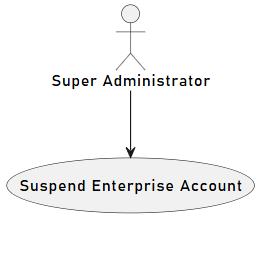
\includegraphics[width=0.4\linewidth,keepaspectratio]{assets/uc_diagrams/uc_suspend_enterprise.png} 
\\ \hline

\end{tabularx}

\vspace{2em}

% ================================================
% Manage Subscription Plans
% ================================================
\begin{tabularx}{\linewidth}{|>{\raggedright\arraybackslash}p{4cm}|>{\raggedright\arraybackslash}X|}
\caption{Use Case Specification: Manage Subscription Plans}
\label{tab:uc-manage-subscription} \\ \hline

\textbf{Field} & \textbf{Details} \\ \hline
Use Case ID & UC-03 \\ \hline
Use Case Name & Manage Subscription Plans \\ \hline
Primary Actor & Super Administrator \\ \hline
Secondary Actor(s) & None \\ \hline

Description &
Defines, modifies, activates, or deactivates subscription plans.
\\ \hline

Preconditions &
Super Administrator is logged in.
\\ \hline

Postconditions &
Subscription plans are updated.
\\ \hline

Main Flow (Basic Flow) &
1. Super Administrator accesses plan management. \newline
2. System displays current plans. \newline
3. Super Administrator modifies plan. \newline
4. System saves changes. \newline
5. System confirms update.
\\ \hline

Alternative Flow(s) &
A1: Create new plan – System prompts for new plan details.
\\ \hline

Exception Flow(s) &
E1: Invalid plan details – System notifies and returns to step 3.
\\ \hline

Use Case Diagram &
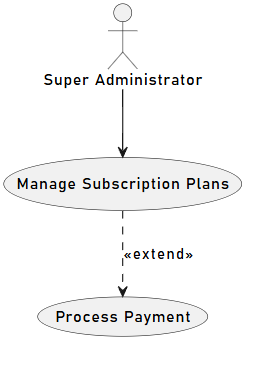
\includegraphics[width=0.4\linewidth,keepaspectratio]{assets/uc_diagrams/uc_manage_subscription.png}
\\ \hline

\end{tabularx}

\vspace{2em}

% ================================================
% View System Dashboard
% ================================================
\begin{tabularx}{\linewidth}{|>{\raggedright\arraybackslash}p{4cm}|>{\raggedright\arraybackslash}X|}
\caption{Use Case Specification: View System Dashboard}
\label{tab:uc-view-dashboard} \\ \hline

\textbf{Field} & \textbf{Details} \\ \hline
Use Case ID & UC-04 \\ \hline
Use Case Name & View System Dashboard \\ \hline
Primary Actor & Super Administrator \\ \hline
Secondary Actor(s) & None \\ \hline

Description &
Displays system-wide metrics and key performance indicators.
\\ \hline

Preconditions &
- Super Administrator is logged in.
\\ \hline

Postconditions &
- System dashboard information is presented.
\\ \hline

Main Flow (Basic Flow) &
1. Super Administrator accesses dashboard. \newline
2. System retrieves and displays data. \newline
3. Super Administrator views information.
\\ \hline

Alternative Flow(s) &
None
\\ \hline

Exception Flow(s) &
E1: No data available – System displays empty dashboard message.
\\ \hline

Use Case Diagram &
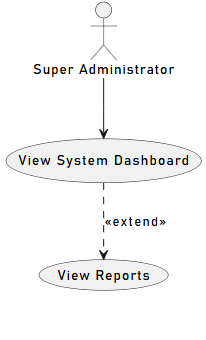
\includegraphics[width=0.4\linewidth,keepaspectratio]{assets/uc_diagrams/uc_view_dashboard.png}
\\ \hline
\end{tabularx}

\vspace{2em}


% ===============================================
% Use Case Diagram: Enterprise Administrator Use Cases
% ===============================================

\paragraph{Enterprise Administrator – Use Case Diagram}

% ================================================
% Register Enterprise
% ================================================
\begin{tabularx}{\linewidth}{|>{\raggedright\arraybackslash}p{4cm}|>{\raggedright\arraybackslash}X|}
\caption{Use Case Specification: Register Enterprise}
\label{tab:uc-register-enterprise} \\ \hline

\textbf{Field} & \textbf{Details} \\ \hline
Use Case ID & UC-05 \\ \hline
Use Case Name & Register Enterprise \\ \hline
Primary Actor & Enterprise Administrator \\ \hline
Secondary Actor(s) & None \\ \hline

Description &
Submits a request to set up a new enterprise environment.
\\ \hline

Preconditions &
- The enterprise does not have an existing account.
\\ \hline

Postconditions &
- Registration request is submitted for approval.
\\ \hline

Main Flow (Basic Flow) &
1. Enterprise Administrator initiates registration. \newline
2. System prompts for enterprise details. \newline
3. Enterprise Administrator provides required details. \newline
4. System validates the details. \newline
5. System submits request for approval.
\\ \hline

Alternative Flow(s) &
A1: Invalid details provided – System notifies of errors and returns to step 3.
\\ \hline

Exception Flow(s) &
E1: Registration fails due to system error – System displays error message and suggests retry.
\\ \hline

Use Case Diagram &
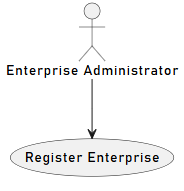
\includegraphics[width=0.4\linewidth,keepaspectratio]{assets/uc_diagrams/uc_register_enterprise.png}
\\ \hline
\end{tabularx}

\vspace{2em}

% ================================================
% Login
% ================================================
\begin{tabularx}{\linewidth}{|>{\raggedright\arraybackslash}p{4cm}|>{\raggedright\arraybackslash}X|}
\caption{Use Case Specification: Login}
\label{tab:uc-login} \\ \hline

\textbf{Field} & \textbf{Details} \\ \hline
Use Case ID & UC-06, UC-14, UC-18 \\ \hline
Use Case Name & Login \\ \hline
Primary Actor & Enterprise Administrator \\ \hline
Secondary Actor(s) & Enterprise Staff, Candidate \\ \hline

Description &
Authenticates a user to access the system based on role.
\\ \hline

Preconditions &
- The user has a registered and approved account.
\\ \hline

Postconditions &
- The user is authenticated and granted role-based access.
\\ \hline

Main Flow (Basic Flow) &
1. User initiates login. \newline
2. System prompts for credentials. \newline
3. User provides credentials. \newline
4. System verifies credentials. \newline
5. System grants access.
\\ \hline

Alternative Flow(s) &
A1: Forgot credentials – System provides recovery option.
\\ \hline

Exception Flow(s) &
E1: Invalid credentials – System displays error and allows retry.
\\ \hline

Use Case Diagram &
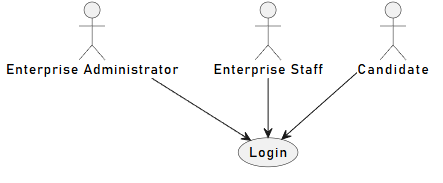
\includegraphics[width=0.6\linewidth,keepaspectratio]{assets/uc_diagrams/uc_login.png}
\\ \hline
\end{tabularx}

\vspace{2em}

% ================================================
% Manage Staff
% ================================================
\begin{tabularx}{\linewidth}{|>{\raggedright\arraybackslash}p{4cm}|>{\raggedright\arraybackslash}X|}
\caption{Use Case Specification: Manage Staff}
\label{tab:uc-manage-staff} \\ \hline

\textbf{Field} & \textbf{Details} \\ \hline
Use Case ID & UC-07 \\ \hline
Use Case Name & Manage Staff \\ \hline
Primary Actor & Enterprise Administrator \\ \hline
Secondary Actor(s) & None \\ \hline

Description &
Creates, modifies, or removes staff accounts and permissions within the enterprise.
\\ \hline

Preconditions &
- Enterprise Administrator is logged in.
\\ \hline

Postconditions &
- Staff list is updated.
\\ \hline

Main Flow (Basic Flow) &
1. Enterprise Administrator selects manage staff. \newline
2. System displays staff list. \newline
3. Enterprise Administrator performs action on staff. \newline
4. System updates the staff information. \newline
5. System confirms changes.
\\ \hline

Alternative Flow(s) &
A1: Assign permissions – System allows setting role-based permissions.
\\ \hline

Exception Flow(s) &
E1: Invalid action – System displays error and returns to step 3.
\\ \hline

Use Case Diagram &
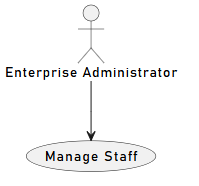
\includegraphics[width=0.4\linewidth,keepaspectratio]{assets/uc_diagrams/uc_manage_staff.png}
\\ \hline
\end{tabularx}

\vspace{2em}

% ================================================
% Create Exam
% ================================================
\begin{tabularx}{\linewidth}{|>{\raggedright\arraybackslash}p{4cm}|>{\raggedright\arraybackslash}X|}
\caption{Use Case Specification: Create Exam}
\label{tab:uc-create-exam} \\ \hline

\textbf{Field} & \textbf{Details} \\ \hline
Use Case ID & UC-08 \\ \hline
Use Case Name & Create Exam \\ \hline
Primary Actor & Enterprise Administrator \\ \hline
Secondary Actor(s) & None \\ \hline

Description &
Creates a new assessment with questions and settings.
\\ \hline

Preconditions &
- Enterprise Administrator is logged in.
\\ \hline

Postconditions &
- New exam is added to the system.
\\ \hline

Main Flow (Basic Flow) &
1. Enterprise Administrator initiates exam creation. \newline
2. System prompts for exam details and questions. \newline
3. Enterprise Administrator provides details. \newline
4. System saves the exam. \newline
5. System confirms creation.
\\ \hline

Alternative Flow(s) &
A1: Set randomization rules – System allows configuring question randomization.
\\ \hline

Exception Flow(s) &
E1: Incomplete details – System notifies and returns to step 3.
\\ \hline

Use Case Diagram &
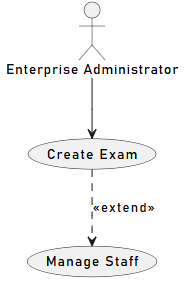
\includegraphics[width=0.4\linewidth,keepaspectratio]{assets/uc_diagrams/uc_create_exam.png}
\\ \hline
\end{tabularx}

\vspace{2em}

% ================================================
% Schedule Exam
% ================================================
\begin{tabularx}{\linewidth}{|>{\raggedright\arraybackslash}p{4cm}|>{\raggedright\arraybackslash}X|}
\caption{Use Case Specification: Schedule Exam}
\label{tab:uc-schedule-exam} \\ \hline

\textbf{Field} & \textbf{Details} \\ \hline
Use Case ID & UC-09 \\ \hline
Use Case Name & Schedule Exam \\ \hline
Primary Actor & Enterprise Administrator \\ \hline
Secondary Actor(s) & None \\ \hline

Description &
Sets timing and availability for an exam.
\\ \hline

Preconditions &
- Enterprise Administrator is logged in. \newline
- Exam exists.
\\ \hline

Postconditions &
- Exam is scheduled.
\\ \hline

Main Flow (Basic Flow) &
1. Enterprise Administrator selects exam to schedule. \newline
2. System prompts for schedule details. \newline
3. Enterprise Administrator provides details. \newline
4. System updates schedule. \newline
5. System confirms scheduling.
\\ \hline

Alternative Flow(s) &
None
\\ \hline

Exception Flow(s) &
E1: Conflicting schedule – System notifies and returns to step 3.
\\ \hline

Use Case Diagram &
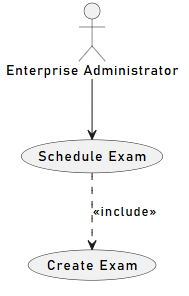
\includegraphics[width=0.4\linewidth,keepaspectratio]{assets/uc_diagrams/uc_schedule_exam.png}
\\ \hline
\end{tabularx}

\vspace{2em}

% ================================================
% Assign Candidates
% ================================================
\begin{tabularx}{\linewidth}{|>{\raggedright\arraybackslash}p{4cm}|>{\raggedright\arraybackslash}X|}
\caption{Use Case Specification: Assign Candidates}
\label{tab:uc-assign-candidates} \\ \hline

\textbf{Field} & \textbf{Details} \\ \hline
Use Case ID & UC-10 \\ \hline
Use Case Name & Assign Candidates \\ \hline
Primary Actor & Enterprise Administrator \\ \hline
Secondary Actor(s) & None \\ \hline

Description &
Assigns candidates to a scheduled exam.
\\ \hline

Preconditions &
- Enterprise Administrator is logged in. \newline
- Exam is scheduled.
\\ \hline

Postconditions &
- Candidates are assigned to the exam.
\\ \hline

Main Flow (Basic Flow) &
1. Enterprise Administrator selects exam. \newline
2. System displays candidate list. \newline
3. Enterprise Administrator selects candidates. \newline
4. System assigns candidates. \newline
5. System confirms assignment.
\\ \hline

Alternative Flow(s) &
A1: Invite new candidates – System allows adding new candidates.
\\ \hline

Exception Flow(s) &
E1: No candidates available – System prompts to add candidates.
\\ \hline

Use Case Diagram &
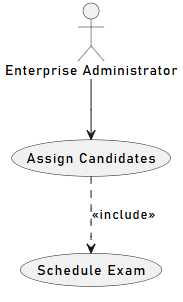
\includegraphics[width=0.4\linewidth,keepaspectratio]{assets/uc_diagrams/uc_assign_candidates.png}
\\ \hline
\end{tabularx}

\vspace{2em}

% ================================================
% View Dashboard
% ================================================
\begin{tabularx}{\linewidth}{|>{\raggedright\arraybackslash}p{4cm}|>{\raggedright\arraybackslash}X|}
\caption{Use Case Specification: View Dashboard}
\label{tab:uc-view-dashboard-enterprise} \\ \hline

\textbf{Field} & \textbf{Details} \\ \hline
Use Case ID & UC-11 \\ \hline
Use Case Name & View Dashboard \\ \hline
Primary Actor & Enterprise Administrator \\ \hline
Secondary Actor(s) & None \\ \hline

Description &
Displays enterprise-specific overview of exams, participants, and results.
\\ \hline

Preconditions &
- Enterprise Administrator is logged in.
\\ \hline

Postconditions &
- Dashboard information is presented.
\\ \hline

Main Flow (Basic Flow) &
1. Enterprise Administrator accesses dashboard. \newline
2. System retrieves and displays data. \newline
3. Enterprise Administrator views information.
\\ \hline

Alternative Flow(s) &
None
\\ \hline

Exception Flow(s) &
E1: No data available – System displays empty dashboard message.
\\ \hline

Use Case Diagram &
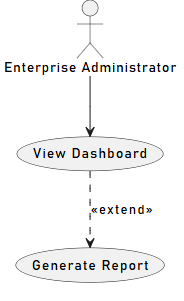
\includegraphics[width=0.4\linewidth,keepaspectratio]{assets/uc_diagrams/uc_view_dashboard_enterprise.png}
\\ \hline
\end{tabularx}

\vspace{2em}

% ================================================
% Generate Report
% ================================================
\begin{tabularx}{\linewidth}{|>{\raggedright\arraybackslash}p{4cm}|>{\raggedright\arraybackslash}X|}
\caption{Use Case Specification: Generate Report}
\label{tab:uc-generate-report} \\ \hline

\textbf{Field} & \textbf{Details} \\ \hline
Use Case ID & UC-12 \\ \hline
Use Case Name & Generate Report \\ \hline
Primary Actor & Enterprise Administrator \\ \hline
Secondary Actor(s) & None \\ \hline

Description &
Produces reports on exam results and analytics for the enterprise.
\\ \hline

Preconditions &
- Enterprise Administrator is logged in. \newline
- Exam data exists.
\\ \hline

Postconditions &
- Report is generated.
\\ \hline

Main Flow (Basic Flow) &
1. Enterprise Administrator requests report. \newline
2. System prompts for report criteria. \newline
3. Enterprise Administrator provides criteria. \newline
4. System generates report. \newline
5. System presents report.
\\ \hline

Alternative Flow(s) &
A1: Analytics report – System includes performance analytics.
\\ \hline

Exception Flow(s) &
E1: Insufficient data – System notifies and suggests alternatives.
\\ \hline

Use Case Diagram &
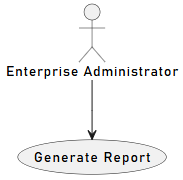
\includegraphics[width=0.4\linewidth,keepaspectratio]{assets/uc_diagrams/uc_generate_report.png}
\\ \hline
\end{tabularx}

\vspace{2em}


% ================================================
% Manage Enterprise Subscription
% ================================================
\begin{tabularx}{\linewidth}{|>{\raggedright\arraybackslash}p{4cm}|>{\raggedright\arraybackslash}X|}
\caption{Use Case Specification: Manage Enterprise Subscription}
\label{tab:uc-manage-enterprise-subscription} \\ \hline

\textbf{Field} & \textbf{Details} \\ \hline
Use Case ID & UC-13 \\ \hline
Use Case Name & Manage Enterprise Subscription \\ \hline
Primary Actor & Enterprise Administrator \\ \hline
Secondary Actor(s) & None \\ \hline

Description &
Upgrades, downgrades, or manages the enterprise's subscription plan.
\\ \hline

Preconditions &
- Enterprise Administrator is logged in.
\\ \hline

Postconditions &
- Subscription is updated.
\\ \hline

Main Flow (Basic Flow) &
1. Enterprise Administrator accesses subscription management. \newline
2. System displays current plan and options. \newline
3. Enterprise Administrator selects change. \newline
4. System processes update. \newline
5. System confirms change.
\\ \hline

Alternative Flow(s) &
A1: Upgrade plan – System enables additional features.
\\ \hline

Exception Flow(s) &
E1: Payment required – System redirects to payment.
\\ \hline

Use Case Diagram &
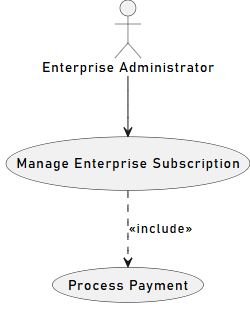
\includegraphics[width=0.4\linewidth,keepaspectratio]{assets/uc_diagrams/uc_manage_enterprise_subscription.png}
\\ \hline
\end{tabularx}

\vspace{2em}


\begin{figure}[H]
\centering
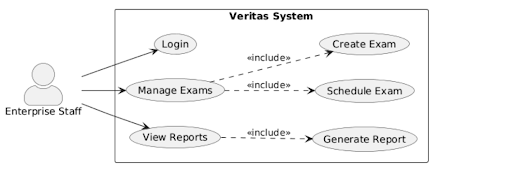
\includegraphics[width=\linewidth,keepaspectratio]{assets/uc_diagrams/uc_enterprise_staff.png}
\caption{Use Case Diagram of Enterprise Staff}
\label{fig:use-case-diagram-enterprise-staff}
\end{figure}
    

% ===============================================
% Use Case Diagram: Enterprise Staff Use Cases
% ===============================================

\paragraph{Enterprise Staff – Use Case Diagram}

% ================================================
% Manage Exams
% ================================================
\begin{tabularx}{\linewidth}{|>{\raggedright\arraybackslash}p{4cm}|>{\raggedright\arraybackslash}X|}
\caption{Use Case Specification: Manage Exams}
\label{tab:uc-manage-exams} \\ \hline

\textbf{Field} & \textbf{Details} \\ \hline
Use Case ID & UC-15 \\ \hline
Use Case Name & Manage Exams \\ \hline
Primary Actor & Enterprise Staff \\ \hline
Secondary Actor(s) & None \\ \hline

Description &
Handles exam creation, scheduling, and management within permissions.
\\ \hline

Preconditions &
- Enterprise Staff is logged in.
\\ \hline

Postconditions &
- Exam is managed.
\\ \hline

Main Flow (Basic Flow) &
1. Enterprise Staff selects exam management. \newline
2. System displays available exams. \newline
3. Enterprise Staff performs action. \newline
4. System updates exam. \newline
5. System confirms changes.
\\ \hline

Alternative Flow(s) &
None
\\ \hline

Exception Flow(s) &
E1: Permission denied – System notifies of lack of access.
\\ \hline

Use Case Diagram &
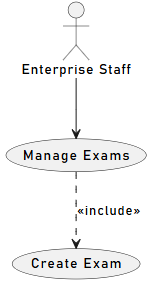
\includegraphics[width=0.4\linewidth,keepaspectratio]{assets/uc_diagrams/uc_manage_exams.png}
\\ \hline
\end{tabularx}

\vspace{2em}

% ================================================
% View Reports
% ================================================
\begin{tabularx}{\linewidth}{|>{\raggedright\arraybackslash}p{4cm}|>{\raggedright\arraybackslash}X|}
\caption{Use Case Specification: View Reports}
\label{tab:uc-view-reports} \\ \hline

\textbf{Field} & \textbf{Details} \\ \hline
Use Case ID & UC-16 \\ \hline
Use Case Name & View Reports \\ \hline
Primary Actor & Enterprise Staff \\ \hline
Secondary Actor(s) & None \\ \hline

Description &
Views reports on exam results and analytics.
\\ \hline

Preconditions &
- Enterprise Staff is logged in. \newline
- Report data exists.
\\ \hline

Postconditions &
- Report is viewed.
\\ \hline

Main Flow (Basic Flow) &
1. Enterprise Staff requests report. \newline
2. System displays report options. \newline
3. Enterprise Staff selects criteria. \newline
4. System presents report. \newline
5. Enterprise Staff views report.
\\ \hline

Alternative Flow(s) &
None
\\ \hline

Exception Flow(s) &
E1: No access to data – System notifies of permissions.
\\ \hline

Use Case Diagram &
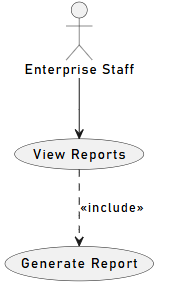
\includegraphics[width=0.4\linewidth,keepaspectratio]{assets/uc_diagrams/uc_view_reports.png}
\\ \hline
\end{tabularx}

\vspace{2em}

\begin{figure}[H]
\centering
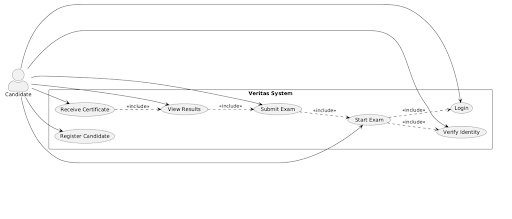
\includegraphics[width=\linewidth,keepaspectratio]{assets/uc_diagrams/uc_candidate.png}
\caption{Use Case Diagram of Candidate}
\label{fig:use-case-diagram-candidate}
\end{figure}

% ================================================
% Use Case Diagram: Candidate Use Cases
% ================================================
\paragraph{Candidate – Use Case Diagram}

% ================================================
% Register Candidate
% ================================================
\begin{tabularx}{\linewidth}{|>{\raggedright\arraybackslash}p{4cm}|>{\raggedright\arraybackslash}X|}
\caption{Use Case Specification: Register Candidate}
\label{tab:uc-register-candidate} \\ \hline

\textbf{Field} & \textbf{Details} \\ \hline
Use Case ID & UC-17 \\ \hline
Use Case Name & Register Candidate \\ \hline
Primary Actor & Candidate \\ \hline
Secondary Actor(s) & None \\ \hline

Description &
Allows a candidate to create an account for assessments.
\\ \hline

Preconditions &
- Candidate does not have an account.
\\ \hline

Postconditions &
- Candidate account is created.
\\ \hline

Main Flow (Basic Flow) &
1. Candidate initiates registration. \newline
2. System prompts for details. \newline
3. Candidate provides details. \newline
4. System validates details. \newline
5. System creates account.
\\ \hline

Alternative Flow(s) &
A1: Use enterprise-issued ID – System verifies ID.
\\ \hline

Exception Flow(s) &
E1: Duplicate account – System notifies and suggests login.
\\ \hline

Use Case Diagram &
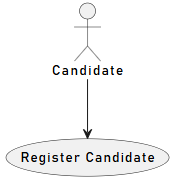
\includegraphics[width=0.4\linewidth,keepaspectratio]{assets/uc_diagrams/uc_register_candidate.png}
\\ \hline
\end{tabularx}

\vspace{2em}

% ================================================
% Verify Identity
% ================================================
\begin{tabularx}{\linewidth}{|>{\raggedright\arraybackslash}p{4cm}|>{\raggedright\arraybackslash}X|}
\caption{Use Case Specification: Verify Identity}
\label{tab:uc-verify-identity} \\ \hline

\textbf{Field} & \textbf{Details} \\ \hline
Use Case ID & UC-19 \\ \hline
Use Case Name & Verify Identity \\ \hline
Primary Actor & Candidate \\ \hline
Secondary Actor(s) & None \\ \hline

Description &
Confirms the candidate's identity during assessment.
\\ \hline

Preconditions &
- Candidate is logged in.
\\ \hline

Postconditions &
- Identity is verified.
\\ \hline

Main Flow (Basic Flow) &
1. Candidate initiates verification. \newline
2. System captures image. \newline
3. Candidate allows capture. \newline
4. System compares image. \newline
5. System confirms verification.
\\ \hline

Alternative Flow(s) &
None
\\ \hline

Exception Flow(s) &
E1: Verification fails – System notifies and allows retry.
\\ \hline

Use Case Diagram &
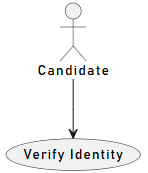
\includegraphics[width=0.4\linewidth,keepaspectratio]{assets/uc_diagrams/uc_verify_identity.png}
\\ \hline
\end{tabularx}

\vspace{2em}

% ================================================
% Start Exam
% ================================================
\begin{tabularx}{\linewidth}{|>{\raggedright\arraybackslash}p{4cm}|>{\raggedright\arraybackslash}X|}
\caption{Use Case Specification: Start Exam}
\label{tab:uc-start-exam} \\ \hline

\textbf{Field} & \textbf{Details} \\ \hline
Use Case ID & UC-20 \\ \hline
Use Case Name & Start Exam \\ \hline
Primary Actor & Candidate \\ \hline
Secondary Actor(s) & None \\ \hline

Description &
Begins the assessment session.
\\ \hline

Preconditions &
- Candidate is assigned to exam. \newline
- Exam is scheduled and available.
\\ \hline

Postconditions &
- Exam session is active.
\\ \hline

Main Flow (Basic Flow) &
1. Candidate selects exam. \newline
2. System checks eligibility. \newline
3. Candidate starts exam. \newline
4. System presents questions. \newline
5. Exam begins.
\\ \hline

Alternative Flow(s) &
A1: Activate monitoring – System starts tracking behavior.
\\ \hline

Exception Flow(s) &
E1: Exam not available – System notifies of schedule.
\\ \hline

Use Case Diagram &
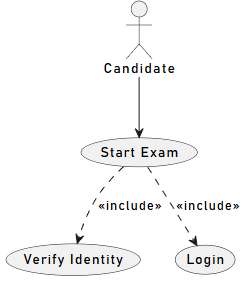
\includegraphics[width=0.4\linewidth,keepaspectratio]{assets/uc_diagrams/uc_start_exam.png}
\\ \hline
\end{tabularx}

\vspace{2em}

% ================================================
% Submit Exam
% ================================================
\begin{tabularx}{\linewidth}{|>{\raggedright\arraybackslash}p{4cm}|>{\raggedright\arraybackslash}X|}
\caption{Use Case Specification: Submit Exam}
\label{tab:uc-submit-exam} \\ \hline

\textbf{Field} & \textbf{Details} \\ \hline
Use Case ID & UC-21 \\ \hline
Use Case Name & Submit Exam \\ \hline
Primary Actor & Candidate \\ \hline
Secondary Actor(s) & None \\ \hline

Description &
Submits answers for grading.
\\ \hline

Preconditions &
- Exam session is active.
\\ \hline

Postconditions &
- Answers are submitted.
\\ \hline

Main Flow (Basic Flow) &
1. Candidate completes answers. \newline
2. System prompts for submission. \newline
3. Candidate confirms submission. \newline
4. System records answers. \newline
5. System ends session.
\\ \hline

Alternative Flow(s) &
A1: Auto-submit on time expiry – System submits automatically.
\\ \hline

Exception Flow(s) &
E1: Incomplete submission – System warns before ending.
\\ \hline

Use Case Diagram &
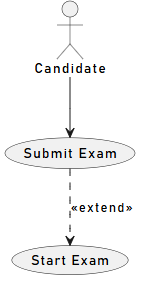
\includegraphics[width=0.4\linewidth,keepaspectratio]{assets/uc_diagrams/uc_submit_exam.png}
\\ \hline
\end{tabularx}

\vspace{2em}

% ================================================
% View Results
% ================================================
\begin{tabularx}{\linewidth}{|>{\raggedright\arraybackslash}p{4cm}|>{\raggedright\arraybackslash}X|}
\caption{Use Case Specification: View Results}
\label{tab:uc-view-results} \\ \hline

\textbf{Field} & \textbf{Details} \\ \hline
Use Case ID & UC-22 \\ \hline
Use Case Name & View Results \\ \hline
Primary Actor & Candidate \\ \hline
Secondary Actor(s) & None \\ \hline

Description &
Displays personal assessment results and feedback.
\\ \hline

Preconditions &
- Exam is submitted.
\\ \hline

Postconditions &
- Results are presented.
\\ \hline

Main Flow (Basic Flow) &
1. Candidate requests results. \newline
2. System retrieves results. \newline
3. Candidate views results and feedback.
\\ \hline

Alternative Flow(s) &
A1: Receive personalized feedback – System provides insights.
\\ \hline

Exception Flow(s) &
E1: Results not ready – System notifies of processing.
\\ \hline

Use Case Diagram &
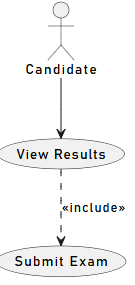
\includegraphics[width=0.4\linewidth,keepaspectratio]{assets/uc_diagrams/uc_view_results.png}
\\ \hline
\end{tabularx}

\vspace{2em}

% ================================================
% Use Case Diagram: Payment System Use Cases
% ================================================
\paragraph{Payment System – Use Case Diagram}
% ================================================
% Process Payment
% ================================================
\begin{tabularx}{\linewidth}{|>{\raggedright\arraybackslash}p{4cm}|>{\raggedright\arraybackslash}X|}
\caption{Use Case Specification: Process Payment}
\label{tab:uc-process-payment} \\ \hline

\textbf{Field} & \textbf{Details} \\ \hline
Use Case ID & UC-24 \\ \hline
Use Case Name & Process Payment \\ \hline
Primary Actor & Payment System \\ \hline
Secondary Actor(s) & None \\ \hline

Description &
Handles payment for subscription changes or plans.
\\ \hline

Preconditions &
- Payment is required for action.
\\ \hline

Postconditions &
- Payment is processed.
\\ \hline

Main Flow (Basic Flow) &
1. The system initiates payment. \newline
2. Payment System processes details. \newline
3. Payment System confirms transaction.
\\ \hline

Alternative Flow(s) &
None
\\ \hline

Exception Flow(s) &
E1: Payment fails – Payment System notifies error.
\\ \hline

Use Case Diagram &
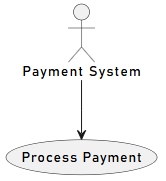
\includegraphics[width=0.4\linewidth,keepaspectratio]{assets/uc_diagrams/uc_process_payment.png}
\\ \hline
\end{tabularx}

\vspace{2em}
